\documentclass[a4paper, 12pt]{article}
\usepackage[utf8]{inputenc}
\usepackage{myshortcuts}
\usepackage{a4wide}
\usepackage{hyperref}
\usepackage[english]{babel}
\usepackage{csquotes}
\usepackage{caption}
\usepackage[style=mla,backend=biber]{biblatex}

\addbibresource{mysources.bib}

\title{
{\large Mathematics Internal Assessment}\\
\bigskip
How can we model percolation mathematically?
}
\author{Jingjie YANG}
\date{October 2018}

\begin{document}
\maketitle

\paragraph{Abstract.}
The phenomenon of percolation in materials science is described, and a mathematical model of percolation on the square lattice $\Z^2$ is presented, in which each edge has a probability of $p \in [0, 1]$ to be open. Whether infinite components of open edges exist and the critical value $p_c$ at which they appear are then considered. It is firstly shown that there exists a unique infinite component, and $0 < p_c < 1$, before concluding that $p_c = \frac{1}{2}$. 

\section*{Introduction}

\begin{figure}[!htb]
    \centering
    \minipage{0.32\textwidth}
    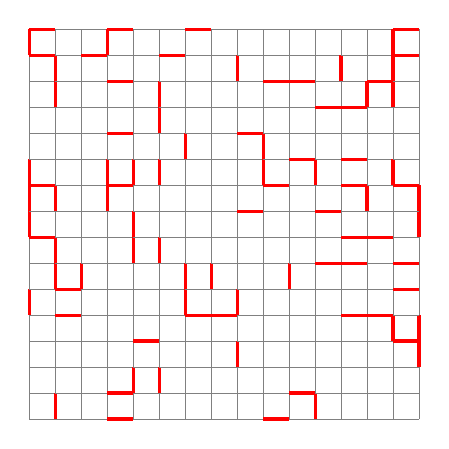
\begin{tikzpicture}
        \def\p{0.2}
        \foreach \x in {0,0.33,...,4.63} {
            \foreach \y in {0,0.33,...,4.63} {
                \pgfmathparse{rnd}
                \ifdim\pgfmathresult pt < \p pt\relax 
                    \draw[red, very thick] (\x, \y) -- (\x, \y + 0.33);
                \else
                    \draw[gray] (\x, \y) -- (\x, \y + 0.33);
                \fi 
                \pgfmathparse{rnd}
                \ifdim\pgfmathresult pt < \p pt\relax
                    \draw[red, very thick] (\x, \y) -- (\x + 0.33, \y);
                \else
                    \draw[gray] (\x, \y) -- (\x + 0.33, \y);
                \fi 
            }
            \pgfmathparse{rnd}
            \ifdim\pgfmathresult pt < \p pt\relax
                \draw[red, very thick] (\x, 4.95) -- (\x + 0.33, 4.95);
            \else
                \draw[gray] (\x, 4.95) -- (\x + 0.33, 4.95);
            \fi
            \pgfmathparse{rnd}
            \ifdim\pgfmathresult pt < \p pt\relax
                \draw[red, very thick] (4.95, \x) -- (4.95, \x + 0.33);
            \else
                \draw[gray] (4.95, \x) -- (4.95, \x + 0.33);
            \fi
        }
    \end{tikzpicture}
    \caption{$p = 0.2$}
    \endminipage\hfill
    \minipage{0.32\textwidth}
    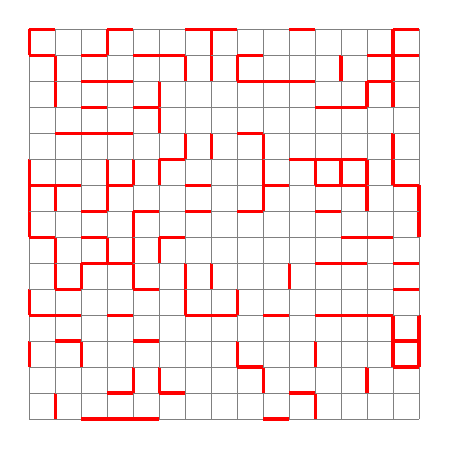
\begin{tikzpicture}
        \def\p{0.3}
        \foreach \x in {0,0.33,...,4.63} {
            \foreach \y in {0,0.33,...,4.63} {
                \pgfmathparse{rnd}
                \ifdim\pgfmathresult pt < \p pt\relax 
                    \draw[red, very thick] (\x, \y) -- (\x, \y + 0.33);
                \else
                    \draw[gray] (\x, \y) -- (\x, \y + 0.33);
                \fi 
                \pgfmathparse{rnd}
                \ifdim\pgfmathresult pt < \p pt\relax
                    \draw[red, very thick] (\x, \y) -- (\x + 0.33, \y);
                \else
                    \draw[gray] (\x, \y) -- (\x + 0.33, \y);
                \fi 
            }
            \pgfmathparse{rnd}
            \ifdim\pgfmathresult pt < \p pt\relax
                \draw[red, very thick] (\x, 4.95) -- (\x + 0.33, 4.95);
            \else
                \draw[gray] (\x, 4.95) -- (\x + 0.33, 4.95);
            \fi
            \pgfmathparse{rnd}
            \ifdim\pgfmathresult pt < \p pt\relax
                \draw[red, very thick] (4.95, \x) -- (4.95, \x + 0.33);
            \else
                \draw[gray] (4.95, \x) -- (4.95, \x + 0.33);
            \fi
        }
    \end{tikzpicture}
    \caption{$p = 0.3$}
    \endminipage\hfill
    \minipage{0.32\textwidth}
    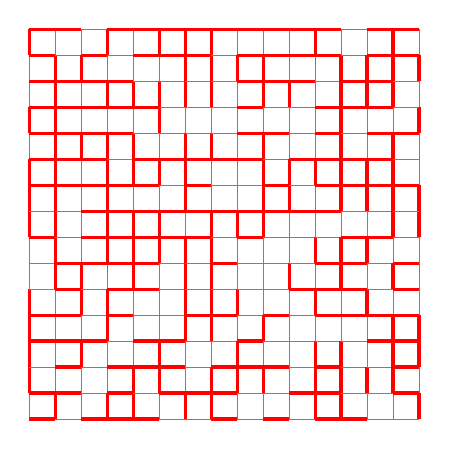
\begin{tikzpicture}
        \def\p{0.6}
        \foreach \x in {0,0.33,...,4.63} {
            \foreach \y in {0,0.33,...,4.63} {
                \pgfmathparse{rnd}
                \ifdim\pgfmathresult pt < \p pt\relax 
                    \draw[red, very thick] (\x, \y) -- (\x, \y + 0.33);
                \else
                    \draw[gray] (\x, \y) -- (\x, \y + 0.33);
                \fi 
                \pgfmathparse{rnd}
                \ifdim\pgfmathresult pt < \p pt\relax
                    \draw[red, very thick] (\x, \y) -- (\x + 0.33, \y);
                \else
                    \draw[gray] (\x, \y) -- (\x + 0.33, \y);
                \fi 
            }
            \pgfmathparse{rnd}
            \ifdim\pgfmathresult pt < \p pt\relax
                \draw[red, very thick] (\x, 4.95) -- (\x + 0.33, 4.95);
            \else
                \draw[gray] (\x, 4.95) -- (\x + 0.33, 4.95);
            \fi
            \pgfmathparse{rnd}
            \ifdim\pgfmathresult pt < \p pt\relax
                \draw[red, very thick] (4.95, \x) -- (4.95, \x + 0.33);
            \else
                \draw[gray] (4.95, \x) -- (4.95, \x + 0.33);
            \fi
        }
    \end{tikzpicture}
    \caption{$p = 0.6$}
    \endminipage\hfill
\end{figure}

\nocite{*}
\printbibliography

\end{document}
